\documentclass[12pt]{article}
% \usepackage[english]{babel}
% \usepackage[utf8x]{inputenc}

\usepackage{graphicx} % Required for inserting images.
\usepackage[margin=25mm]{geometry}
\parskip 4.2pt  % Sets spacing between paragraphs.
% \renewcommand{\baselinestretch}{1.5}  % Uncomment for 1.5 spacing between lines.
\parindent 8.4pt  % Sets leading space for paragraphs.
\usepackage{caption}
\usepackage{amsmath}
\usepackage{amsfonts}
\usepackage{amssymb}
\usepackage{listings}
\usepackage{siunitx}
\usepackage{verbatim}
\usepackage{hyperref} % Required for inserting clickable links.
\usepackage{natbib} % Required for APA-style citations.
\usepackage{titling}

\geometry{a4paper, margin=1in}

\begin{document}

\begin{titlepage}
    \begin{center}
        
\includegraphics[width=0.3\linewidth]{HU logo.jpg} 
        \vspace{1cm}

        \LARGE
        \textbf{RISC V Pipelined Processor}

        \vspace{1.5cm}
        \Large
        \textbf{Final Report}

        \vspace{2cm}
        \large
        \textbf{Submitted by:}\\
        Laiba Ahmed \\
        Meesum Abbas \\
        Raahim Hashmi \\

        \vspace{0.5cm}
        \large
        \textbf{Research Assistant:}\\
        Maham Tabassum

        \vspace{0.5cm}
        \large
       \textbf{ Course Instructor:}\\
       Ahmed Ali Mustansir

        \vspace{1cm}
        \large
        Computer Science \\ 
        Habib University\\
        Spring Semester'24

        \vspace{1cm}
        \large
        Date: \today 

        \vfill
        \small
        \textit{A report submitted in fulfillment\\
        of the requirements for the lab project\\ of 
        CE/CS - 321/330: Computer Architecture}

    \end{center}
\end{titlepage}
\tableofcontents

\newpage

\section{Introduction}
For our final project, we were tasked with creating a 5-stage pipelined RISC-V processor capable of properly executing a bubble sort algorithm. Following are the main tasks associated with achieving this goal:

\begin{enumerate}
    \item Enhancing capability of our lab 11 processor to accommodate instructions needed for bubble sort.
    \item Encoding the bubble sort assembly code into instruction memory and testing it on the processor.
    \item Pipelining the processor by introducing pipeline stage registers, forwarding unit, and hazard detection to produce stall and flush
    \item Comparing the performance of the bubble sort algorithm on the pipelined processor versus the single cycle processor
    
\end{enumerate}

\section{Task 1}
    \subsection{Modifying the existing processor}
        We modified our lab 11 processor to perform logical shift left immediate (\textit{slli}) and branch less than (\textit{blt}) operations to accommodate the bubble sort. \textit{slli} was implemented by producing the required \textit{Operation} signal from \textit{ALU\_Control} and performing the shift left operation in \textit{ALU\_64\_bit}. \textit{blt} was implemented by creating a \textit{branchOp} signal which is low when the operation is \textit{beq} and high when it is \textit{blt}. This, along with \textit{branch}, \textit{Zero}, and a new signal, \textit{Less}, from \textit{ALU\_64\_bit} was used in a simple equation (stored in \textit{var3}) to determine when to branch.
        
\newpage

    \subsection{Bubble Sort Encoding and Testing}
        We modified our bubble sort algorithm\ref{fig:1} to work with a double array and encoded it into the instruction memory. We used the stack in our algorithm and initialized the stack pointer with 92 in \textit{RegisterFile}. Data memory was initialized with the following values: [2,3,0,5,256,4,13,3]. Figures \ref{fig:2} and \ref{fig:3} show the unsorted array and sorted array outputs. Note that each element of the array occupies eight memory locations i.e. 64 bits with the highest index of the highest memory location indicating MSB.\\
        
        \begin{figure}
            \centering
            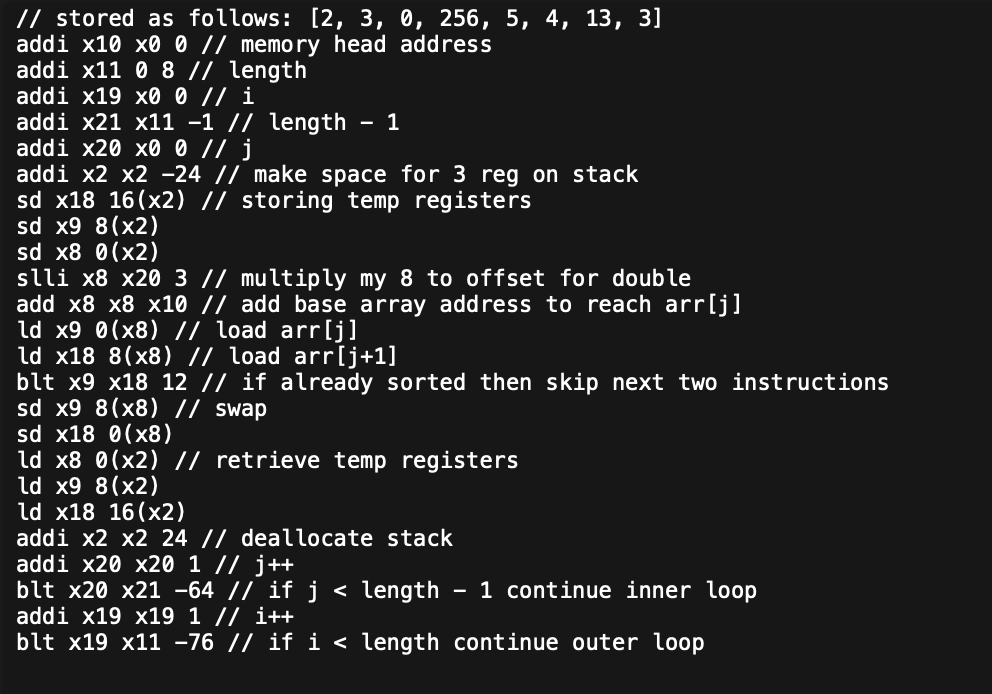
\includegraphics[width=\textwidth]{bubbleSort.png}
            \caption{Bubble Sort Assembly Code}
            \label{fig:1}
        \end{figure}

        \begin{figure}
            \centering
            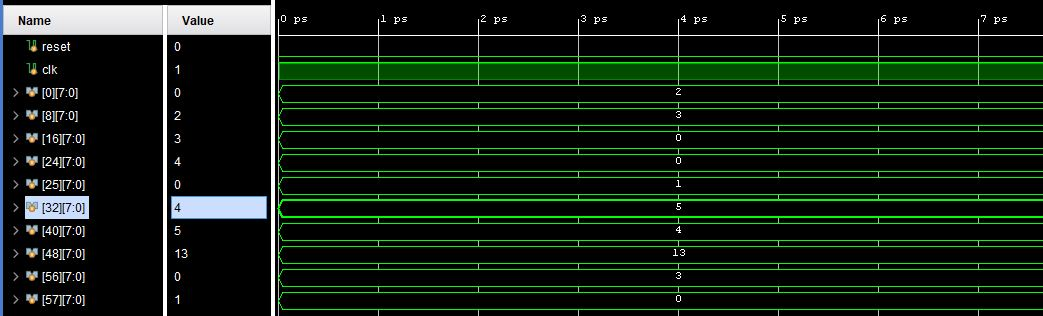
\includegraphics[width=\textwidth]{unsorted.JPG}
            \caption{Unsorted Array}
            \label{fig:2}
        \end{figure}

        \begin{figure}
            \centering
            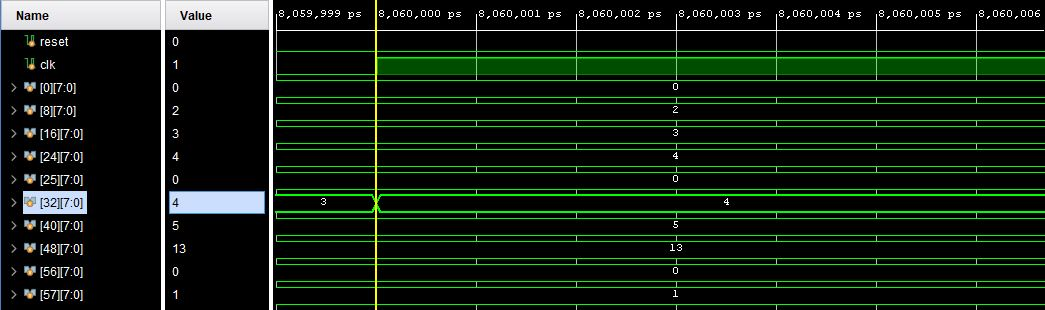
\includegraphics[width=\textwidth]{sorted.JPG}
            \caption{Sorted Array}
            \label{fig:3}
        \end{figure}

\section{Task 2}
    \subsection{Pipelining the processor}

    Once the single cycle processor was functioning properly, we set out to pipeline the processor. For this task we started off by first creating the four pipeline stage registers i.e. \textit{ID\_ID\_Reg, ID\_EXE\_Reg, EXE\_MEM\_Reg, MEM\_WB\_Reg}. We carefully made the proper connections by following the course textbook. We then ran some individual instructions on the processor to ensure it was functioning properly.
    
\newpage

\subsection{Forwarding Unit}

    For implementing the forwarding unit, we used the conditions from the course textbook and made the required connections. Once it was implemented, we ran a couple of dependent instructions and observed they were functioning properly.

\section{Task 3}
    \subsection{Data Hazard Detection}
        In order to deal with the data hazards, we created a hazard detection unit and followed the conditions stated in the course textbook and made the required connections. Once a data hazard was detected, a stall was sent and the outputs for \textit{Program\_Counter} and \textit{IF\_ID\_Reg} would retain their value and all output control signals from \textit{Control\_Unit} would become low, essentially acting as a NOP instruction.

    \subsection{Control Hazard Detection}
        For the control hazards, we used \textit{var3} to act as a signal to flush the \textit{IF\_ID\_Reg, ID\_EX\_REG,} and \textit{EX\_MEM\_Reg} when a branch was detected.

    \subsection{Bubble Sort on Pipelined Processor}
        We then ran our bubble sort instructions on the pipelined processor and figure \ref{fig:4} shows the results. As can be seen, the bubble sort is functioning properly (the unsorted array is the same as figure \ref{fig:1}).

      
    \begin{figure}
        \centering
        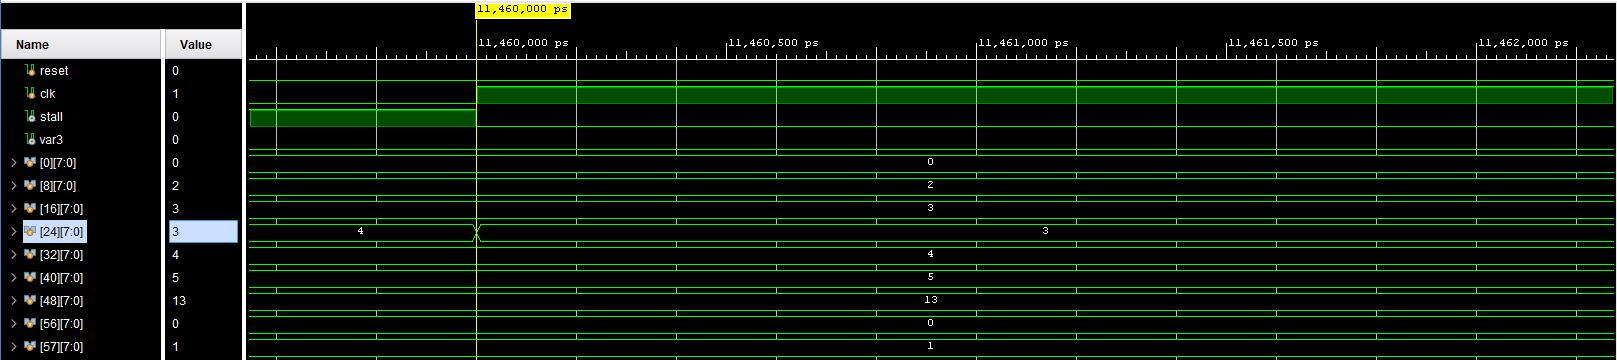
\includegraphics[width=\textwidth]{success.JPG}
        \caption{Task 3 Bubble Sort Result}
        \label{fig:4}
    \end{figure}
    
\newpage

\section{Performance Comparison}
    The pipelined processor that we made is slower than the non-pipelined equivalent. Normally, pipelined processors do take more clock cycles than regular processors; however, their clock is much shorter which makes them faster. In our case, we have kept the clock the same as the regular processor and not according to the duration of the longest pipeline stage as we should have, which makes the non-pipelined version faster simply because of less clock cycles.

\section{Challenges}
    We faced a number of challenges. Initially during forwarding, we had some issues where the data was being forwarded a clock cycle too late which were resolved by removing the clock from the \textit{RegisterFile} as we already had a clock-activated \textit{MEM\_WB\_Reg}. In hazard detection, we had some issues with the stall being activated too late which were resolved by some trial and error on what data fields should be held and what should be zero.

\section{Task Division}
    \begin{itemize}
        \item Laiba: Task 3 (Hazard Detection)
        \item Meesum: Task 2 (Pipelining and Forwarding Unit)
        \item Raahim: Task 1 (Non-pipelined), debbugging and testing tasks 2 and 3
    \end{itemize}
    
    

\section{Conclusion}
    Building the processor and overcoming the challenges that came with it was an overall satisfying and fulfilling experience. This project furthered our understanding of Verilog and enabled us to apply our theoretical knowledge of computer architecture in a worthwhile project.

\section{References}

[1] Book. \textit{Course Book}. Computer Organization and Design: The Hardware/Software Interface RISC-V Edition by David A. Patterson, John L. Hennessy

\section{Appendix}
The GitHub link for our project can be found \href{https://github.com/RaahimHash/Pipelined-RISC-V-Processor}{here}.

    
\end{document}
